\documentclass[submit]{../harvardml}
\usepackage{../common}

\course{CS1810-S26}
\assignment{Homework \#2}
\duedate{February 27, 2026 at 11:59 PM}

\usepackage[OT1]{fontenc}
\usepackage[colorlinks,citecolor=blue,urlcolor=blue]{hyperref}
\usepackage{graphicx}
\usepackage{subcaption}
\usepackage{fullpage}
\usepackage{amsmath}
\usepackage{todonotes}
\usepackage{amssymb}
\usepackage{framed}
\usepackage{color}
\usepackage{soul}
\usepackage{todonotes}
\usepackage{listings}
\usepackage{enumitem}
\usepackage{bm}
\usepackage{bbm}
\usepackage{float}


\newcommand{\B}{\text{B}}
\newcommand{\Beta}{\text{Beta}}

\usepackage[mmddyyyy,hhmmss]{datetime}

\definecolor{verbgray}{gray}{0.9}

\lstnewenvironment{csv}{%
  \lstset{backgroundcolor=\color{verbgray},
  frame=single,
  framerule=0pt,
  basicstyle=\ttfamily,
  columns=fullflexible}}{}


%%%%%%%%%%%%%%%%%%%%%%%%%%%%%%%%%%%%%%%%%%%
%% Solution environment
\usepackage{xcolor}
\newenvironment{solution}{
    \vspace{2mm}
    \color{blue}\noindent\textbf{Solution}:
}{}
%%%%%%%%%%%%%%%%%%%%%%%%%%%%%%%%%%%%%%%%%%%


\begin{document}

\begin{center}
  {\Large Classification and Bias-Variance Trade-offs}\\
\end{center}

\subsection*{Introduction}

This homework is about classification, bias-variance trade-offs, and
uncertainty quantification.

The datasets that we will be working with relate to astronomical observations and loan applicants
The first dataset, found at \verb|data/planet-obs.csv|,
contains information on whether a planet was observed (as a binary
variable) at given points in time. This will be used in Problem 1. The
second dataset, available at \verb|data/hr.csv|, details different
loan applicants and their measured debt to income ratio and credit score. You will
work with this data in Problem 3.

As a general note, for classification problems we imagine that we have
the input matrix $\boldX \in \reals^{N \times D}$ (or perhaps they
have been mapped to some basis $\bm{\Phi}$, without loss of
generality) with outputs now ``one-hot encoded."  This means that if
there are~$K$ output classes, rather than representing the output
label $y$ as an integer~${1,2,\ldots,K}$, we represent $\boldy$ as a
``one-hot" vector of length~$K$. A ``one-hot" vector is defined as
having every component equal to 0 except for a single component which
has value equal to 1.  For example, if there are $K = 7$ classes and a
particular data point belongs to class 3, then the target vector for
this data point would be~$\boldy = [0,0,1,0,0,0,0]$.  We will define
$C_1$ to be the one-hot vector for the 1st class, $C_2$ for the 2nd
class, etc.  Thus, in the previous example $\boldy = C_3$. If there
are $K$ total classes, then the set of possible labels is $\{C_1
  \ldots C_K \} = \{C_k\}_{k=1}^K$.  Throughout the assignment we will
assume that each label $\boldy \in \{C_k\}_{k=1}^K$ unless otherwise
specified. The most common exception is the case of binary
classification ($K = 2$), in which case labels are the typical
integers $y \in \{0, 1\}$.

\subsection*{Resources and Submission Instructions}

In problems 1 and 3, you may use \texttt{numpy} or \texttt{scipy}, but not \texttt{scipy.optimize} or \texttt{sklearn}. Example code is given in the provided notebook. In past years, students have reported numerical stability issues for problem 3 and sometimes problem 1; we encourage students to not worry too much about this, as we are mindful of this in grading, but we recommend trying to run your code on \textbf{Google Colab} if you encounter issues (since this has resolved the issue for many students in the past).

Please type your solutions after the corresponding problems using this \LaTeX\ template, and start each problem on a new page. Please submit the writeup PDF to the Gradescope assignment `HW2'. Remember to assign pages for each question. \textbf{You must include any plots in your writeup PDF.} Please submit your \LaTeX file and code files to the Gradescope assignment `HW2 - Supplemental.' The supplemental files will only be checked in special cases, e.g. honor code issues, etc. Your files should be named in the same way as we provide them in the repository, e.g. \texttt{hw2.pdf}, etc.


\newpage
%%%%%%%%%%%%%%%%%%%%%%%%%%%%%%%%%%%%%%%%%%%%%
% Problem 1
%%%%%%%%%%%%%%%%%%%%%%%%%%%%%%%%%%%%%%%%%%%%%

\begin{problem}[Exploring Bias-Variance and Uncertainty, 30pts]
In this problem, we will explore the bias and variance of a few
different model classes when it comes to logistic regression, use cross validation for model selection, and
investigate two sources of predictive uncertainty in a synthetic
(made-up) scenario.

We are using a powerful telescope in the northern hemisphere to gather
measurements of some planet of interest. At certain times however, our
telescope is unable to detect the planet due to its positioning around
its star.  The data in \verb|data/planet-obs.csv| records the
observation time in the ``Time" column and whether the planet was
detected in the ``Observed" column (with the value 1 representing that
it was observed).  These observations were taken over a dark, clear
week, which is representative of the region.  Since telescope time is
expensive, we would like to build a model to help us schedule and find
times when we are likely to detect the planet.

\begin{enumerate}
\item Before we begin fitting any models, let us first derive the mathematical explanation for the bias-variance tradeoff. Let $\mathcal{D}$ denote the training dataset, while $\mathbf{x}$ is a fixed input (not in $\mathcal{D}$). Suppose the labels are generated via $$y = f(\mathbf{x}) + \varepsilon$$ where $f(\mathbf{x})$ is the true regression function and $\varepsilon$ is a noise term with $\mathbb{E}[\varepsilon|\mathbf{x}] = 0$ and $\text{Var}(\varepsilon|\mathbf{x}) = \sigma^2$. We'll denote the predictor learned from $\mathcal{D}$ as $\hat f_\mathcal{D}(\mathbf{x})$. Then, we have the prediction error as $$\text{MSE} = \mathbb{E}_{\mathcal{D}, y|\mathbf{x}}[(y - \hat f_\mathcal{D}(\mathbf{x}))^2]$$ We will see that this error decomposes into a noise term, a bias term, and a variance term. \begin{enumerate}
    \item Show that the expression for MSE above decomposes into $$\mathbb{E}_{y|\mathbf{x}}[(y - f(\mathbf{x}))^2] + \mathbb{E}_\mathcal{D}[(f(\mathbf{x}) - \hat f_\mathcal{D}(\mathbf{x}))^2] + \text{\{third term\}}$$ Hint: Add and subtract $f(\mathbf{x})$.

    \item Show that the third term from our final expression in part (b) simplifies to 0. Hint: Use Adam's Law/Law of Total Expectation.

    \item Show that the first term from our final expression in part (b) represents the noise in our data, i.e. $\mathbb{E}_{y|\mathbf{x}}[(y - f(\mathbf{x}))^2] = \sigma^2$.

    \item Define the average predictor $\bar f(\mathbf{x}) = \mathbb{E}_\mathcal{D}[\hat f_\mathcal{D}(\mathbf{x})]$. Now show that the the second term from our final expression in part (b) represents the squared bias plus variance, i.e. $\mathbb{E}_\mathcal{D}[(f(\mathbf{x}) - \hat f_\mathcal{D}(\mathbf{x}))^2] = (f(\mathbf{x}) - \bar f(\mathbf{x}))^2 + \mathbb{E}_\mathcal{D}[(\bar f(\mathbf{x}) - \hat f_\mathcal{D}(\mathbf{x}))^2]$.
\end{enumerate}

  \item Now let's explore the use of different bases to model our data. First, randomly split the data into 10 mini-datasets of size $N = 30$. We will use three different basis functions to model the data. We implemented basis 1 as $[1,t]$, where t is the data to help you get started. Then, choose two basis functions, which you'll use to transform the input data in the regression. (Hint: Examples of such basis functions were given in Lecture 2.) \textbf{Please write your chosen basis functions in the written section of your submission for this part of the question. }

  For each of these bases, fit a logistic regression model using sigmoid($\boldw^\top \boldsymbol\phi(t)$) to each dataset by using gradient descent to
        minimize the negative log-likelihood.  This means you will be
        running gradient descent 10 times for each basis, once for each
        dataset.

        Use the given starting values of $\boldw$ and a learning rate of $\eta=0.001$, take 1,000 update
        steps for each gradient descent run, and make sure to average the
        gradient over the data points at each step. These parameters,
        while not perfect, will ensure your code runs reasonably quickly.

  \item After consulting with a domain expert, we find that the probability of observing the planet is periodic as the planet revolves around its star---we are more likely to observe the planet when it is in front of its star than when it is behind it. In fact, the expert determines that observation follows the generating process $y \sim \text{Bern}(f(t))$, where $f(t) = 0.4 \times \cos(1.1t + 1) + 0.5$ for $t \in [0, 6]$ and $y \in \{0,1\}$. Note that we, the modelers, do not usually see the true data distribution. Knowledge of the true $f(t)$ is only exposed in this problem to allow for verification of the true bias.

        Use the given code to plot the true process versus your learned models. Include your plots in your solution PDF.

        \textbf{In no more than 5 sentences}, explain how bias and variance are reflected in the 3 types of curves on the graphs.  How do the fits of the individual and mean prediction functions change?  Keeping in mind that none of the model classes match the true generating process exactly, discuss the extent to which each of the bases approximates the true process.


    \item If we were to increase the size of each dataset drawn from $N = 30$ to a larger number, how would the bias and variance change for each basis? Why might this be the case? You may experiment with generating your own data that follows the true process and plotting the results, but this is \textbf{not} necessary. \textbf{Your response should not be longer than 5 sentences}.

    \item Consider the test point $t = 0.1$. Using your models trained on basis $\boldsymbol\phi_3$, report the predicted probability of observation of the \textit{first} model (the model trained on the first 30 data points). How can we interpret this probability as a measure of uncertainty? Then, compute the variance of the classification probability over your 10 models at the same point $t = 0.1$. How does this measurement capture another source of uncertainty, and how does this differ from the uncertainty represented by the classification probability? Repeat this process (reporting the first model's classification probability and the variance over the 10 models) for the point $t = 3.2$.

          Compare the uncertainties and their sources at times $t=0.1$ and $t=3.2$.

    \item We now need to make some decisions about when to request time on
          the telescope.  The justifications of your decisions will be sent to
          your funding agency, which will determine whether you will be
          allocated funds to use the telescope for your project. You seek out a team that has used the alternative telescope
                  for observing this planet, and they provide you their observation
                  file \verb|data/planet-obs-alternate.csv|.
                  Compare the observations from your telescope to theirs.  What
                  seems to be happening?  What might be an appropriate model for
                  this? Your funding agency asks you to refit your models on these
                  new data.  Do you think this is a reasonable ask, and if so, how
                  will it help you make better decisions about when to request
                  viewing time?  If not, why do you think the additional modeling
                  will not help? You do \emph{not} need to do any modeling; answer this question in \textbf{no more than 10 lines}. We are looking for your reasoning; there may be
          more than one valid answer.


      \item In part 1, we have selected 3 possible bases to use as features when training a model. This gave us 3 possible models. In this part, we will choose the right learning algorithm by using cross validation. Take your dataset split and train 10 models for each basis, using 9 of the chunks for training and 1 of the chunks for validation. Compare the average error across the 10 folds for the 3 bases. Which basis performs the best? Why do you think it performs the best?


  \end{enumerate}
\end{problem}

\newpage

\begin{solution}
\begin{enumerate}

%%%%%%%%%%%%%%%%%%%%%%%%%%%%%%%%%%%%%%%%%%%%%%%%%%%%%%%%%%%%%%%%%%%%%% 1.1
\item
\begin{enumerate}

\item
Add and subtract $f(\mathbf x)$ inside the square:
\[
  y - \hat f_{\mathcal D}(\mathbf x)
  = \underbrace{\big(y - f(\mathbf x)\big)}_{\text{depends only on }y}
  + \underbrace{\big(f(\mathbf x) - \hat f_{\mathcal D}(\mathbf x)\big)}_{\text{depends only on }\mathcal D}.
\]
Squaring and taking $\mathbb E_{\mathcal D, y|\mathbf x}$ of all three resulting terms,
\begin{align*}
  \text{MSE}
  &= \mathbb E_{\mathcal D, y|\mathbf x}\Big[\big(y-f(\mathbf x)\big)^2\Big]
   + \mathbb E_{\mathcal D, y|\mathbf x}\Big[\big(f(\mathbf x)-\hat f_{\mathcal D}(\mathbf x)\big)^2\Big]
   + 2\,\mathbb E_{\mathcal D, y|\mathbf x}\Big[\big(y-f(\mathbf x)\big)\big(f(\mathbf x)-\hat f_{\mathcal D}(\mathbf x)\big)\Big] \\[2pt]
  &= \underbrace{\mathbb E_{y|\mathbf x}\Big[\big(y-f(\mathbf x)\big)^2\Big]}_{\text{(c): noise}}
   + \underbrace{\mathbb E_{\mathcal D}\Big[\big(f(\mathbf x)-\hat f_{\mathcal D}(\mathbf x)\big)^2\Big]}_{\text{(d): bias}^2+\text{variance}}
   + \underbrace{2\,\mathbb E_{\mathcal D, y|\mathbf x}\Big[\big(y-f(\mathbf x)\big)\big(f(\mathbf x)-\hat f_{\mathcal D}(\mathbf x)\big)\Big]}_{\text{(b): }=\,0} .
\end{align*}
In the first term the integrand does not involve $\mathcal D$, so the expectation over
$\mathcal D$ drops out; in the second the integrand does not involve $y$, so the
expectation over $y|\mathbf x$ drops out. $\blacksquare$

\item
Apply the law of total expectation, conditioning on the training set $\mathcal D$:
\[
  \mathbb E_{\mathcal D, y|\mathbf x}\Big[\big(y-f(\mathbf x)\big)\big(f(\mathbf x)-\hat f_{\mathcal D}(\mathbf x)\big)\Big]
  = \mathbb E_{\mathcal D}\Big[\;\mathbb E_{y|\mathbf x}\Big[\big(y-f(\mathbf x)\big)\big(f(\mathbf x)-\hat f_{\mathcal D}(\mathbf x)\big)\;\Big|\;\mathcal D\Big]\Big].
\]
Conditional on $\mathcal D$ the quantity $f(\mathbf x) - \hat f_{\mathcal D}(\mathbf x)$ is a
constant, so it factors out of the inner expectation:
\[
  = \mathbb E_{\mathcal D}\Big[\big(f(\mathbf x)-\hat f_{\mathcal D}(\mathbf x)\big)\;
      \mathbb E_{y|\mathbf x}\big[\,y - f(\mathbf x) \;\big|\; \mathcal D\,\big]\Big].
\]
The test point $\mathbf x$ is \emph{not} in $\mathcal D$, so the fresh label $y$ at
$\mathbf x$ is independent of $\mathcal D$, and
\[
  \mathbb E_{y|\mathbf x}\big[\,y - f(\mathbf x)\;\big|\;\mathcal D\,\big]
  = \mathbb E_{y|\mathbf x}\big[\,y - f(\mathbf x)\,\big]
  = \mathbb E\big[f(\mathbf x) + \varepsilon - f(\mathbf x)\,\big|\,\mathbf x\big]
  = \mathbb E[\varepsilon \,|\, \mathbf x] = 0 .
\]
Every term in the outer expectation is therefore zero, so the whole cross term
vanishes. $\blacksquare$

\item
Substituting $y = f(\mathbf x) + \varepsilon$,
\[
  \mathbb E_{y|\mathbf x}\Big[\big(y - f(\mathbf x)\big)^2\Big]
  = \mathbb E\big[\varepsilon^2 \,\big|\, \mathbf x\big]
  = \operatorname{Var}(\varepsilon \,|\, \mathbf x) + \big(\mathbb E[\varepsilon\,|\,\mathbf x]\big)^2
  = \sigma^2 + 0^2 = \sigma^2 .
\]
This is the \emph{irreducible} error: it involves no model at all, so no choice of
$\hat f_{\mathcal D}$ can reduce it. $\blacksquare$

\item
Add and subtract the average predictor $\bar f(\mathbf x) = \mathbb E_{\mathcal D}[\hat f_{\mathcal D}(\mathbf x)]$:
\[
  f(\mathbf x) - \hat f_{\mathcal D}(\mathbf x)
  = \big(f(\mathbf x) - \bar f(\mathbf x)\big) + \big(\bar f(\mathbf x) - \hat f_{\mathcal D}(\mathbf x)\big).
\]
Squaring and taking $\mathbb E_{\mathcal D}$,
\[
  \mathbb E_{\mathcal D}\Big[\big(f(\mathbf x)-\hat f_{\mathcal D}(\mathbf x)\big)^2\Big]
  = \big(f(\mathbf x)-\bar f(\mathbf x)\big)^2
  + 2\big(f(\mathbf x)-\bar f(\mathbf x)\big)\,\mathbb E_{\mathcal D}\big[\bar f(\mathbf x)-\hat f_{\mathcal D}(\mathbf x)\big]
  + \mathbb E_{\mathcal D}\Big[\big(\bar f(\mathbf x)-\hat f_{\mathcal D}(\mathbf x)\big)^2\Big],
\]
where the first term came out of the expectation because both $f(\mathbf x)$ and
$\bar f(\mathbf x)$ are deterministic given $\mathbf x$. The cross term vanishes by the
definition of $\bar f$:
\[
  \mathbb E_{\mathcal D}\big[\bar f(\mathbf x)-\hat f_{\mathcal D}(\mathbf x)\big]
  = \bar f(\mathbf x) - \mathbb E_{\mathcal D}\big[\hat f_{\mathcal D}(\mathbf x)\big]
  = \bar f(\mathbf x) - \bar f(\mathbf x) = 0 .
\]
Hence
\[
  \mathbb E_{\mathcal D}\Big[\big(f(\mathbf x)-\hat f_{\mathcal D}(\mathbf x)\big)^2\Big]
  = \underbrace{\big(f(\mathbf x)-\bar f(\mathbf x)\big)^2}_{\text{squared bias}}
  + \underbrace{\mathbb E_{\mathcal D}\Big[\big(\bar f(\mathbf x)-\hat f_{\mathcal D}(\mathbf x)\big)^2\Big]}_{\text{variance}} . \qquad \blacksquare
\]
Combining (a)--(d): $\text{MSE} = \sigma^2 + \text{bias}^2 + \text{variance}$.

\end{enumerate}

%%%%%%%%%%%%%%%%%%%%%%%%%%%%%%%%%%%%%%%%%%%%%%%%%%%%%%%%%%%%%%%%%%%%%% 1.2
\item
The data were shuffled once (seed $181$) and split into $10$ disjoint mini-datasets
of $N = 30$. The three bases form a polynomial ladder of increasing capacity:
\[
  \bphi_1(t) = \begin{bmatrix}1 \\ t\end{bmatrix}, \qquad
  \bphi_2(t) = \begin{bmatrix}1 \\ t \\ t^2\end{bmatrix}, \qquad
  \bphi_3(t) = \begin{bmatrix}1 \\ t \\ t^2 \\ t^3 \\ t^4 \\ t^5\end{bmatrix}.
\]
That is, $\bphi_2$ is the quadratic basis and $\bphi_3$ the degree-$5$ polynomial
basis (both include the bias term). For each basis, a logistic regression model
$\sigma(\boldw^\top\bphi(t))$ was fit to each of the $10$ mini-datasets by gradient
descent on the negative log-likelihood, starting from $\boldw = \bzero$, with
$\eta = 0.001$, $1{,}000$ steps, and the gradient averaged over data points:
\[
  \nabla_{\boldw}\,\text{NLL}(\boldw) = \frac1N\,\bphi(\mathbf t)^\top\!\big(\sigma(\bphi(\mathbf t)\boldw) - \mathbf y\big).
\]

%%%%%%%%%%%%%%%%%%%%%%%%%%%%%%%%%%%%%%%%%%%%%%%%%%%%%%%%%%%%%%%%%%%%%% 1.3
\item
\begin{figure}[H]
\centering
\begin{subfigure}{0.49\textwidth}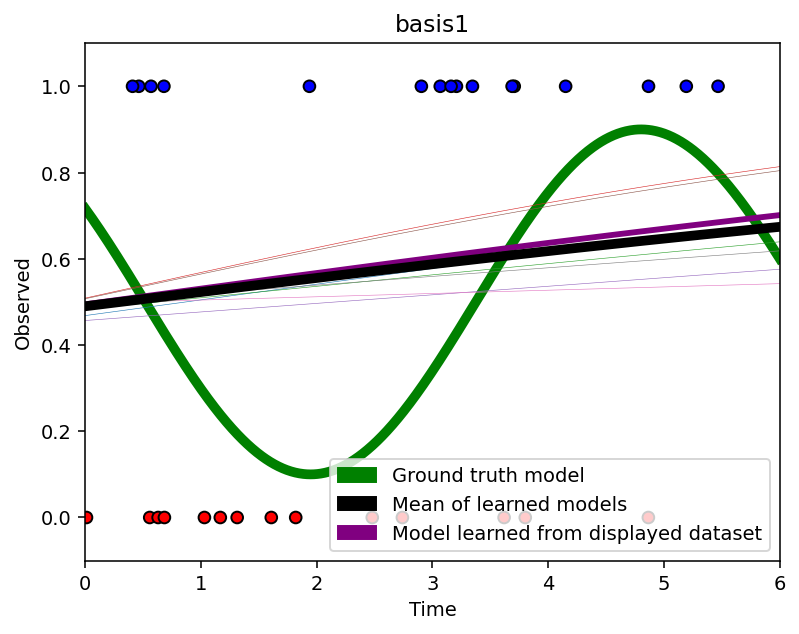
\includegraphics[width=\textwidth]{img_output/basis1.png}\end{subfigure}
\begin{subfigure}{0.49\textwidth}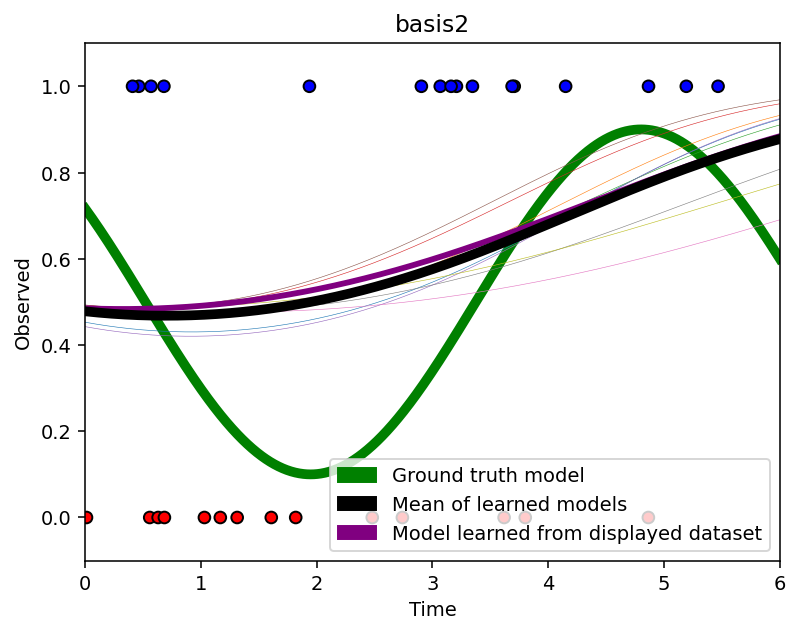
\includegraphics[width=\textwidth]{img_output/basis2.png}\end{subfigure}
\\[4pt]
\begin{subfigure}{0.49\textwidth}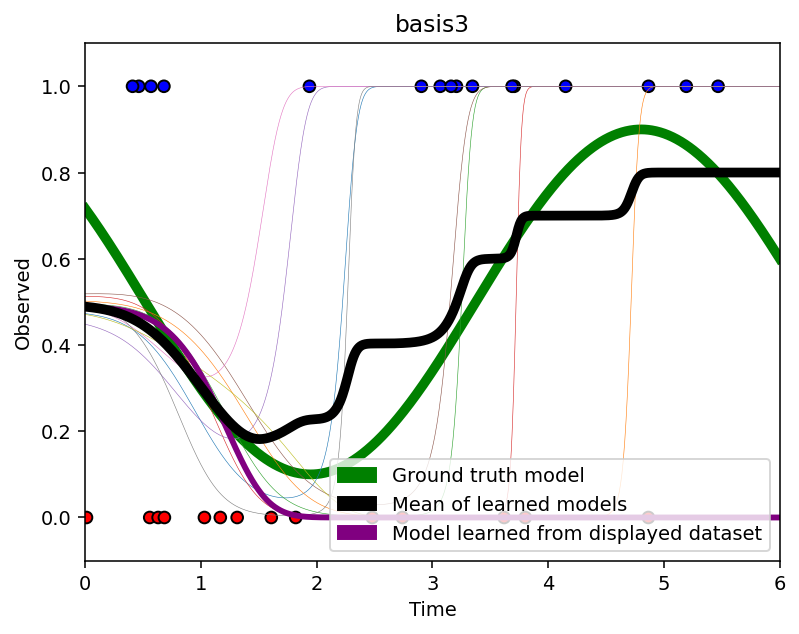
\includegraphics[width=\textwidth]{img_output/basis3.png}\end{subfigure}
\end{figure}

\noindent Measured against the true $f(t)$ on a grid over $[0,6]$:
\begin{center}
\begin{tabular}{lcc}
  \hline
  Basis & avg.\ squared bias & avg.\ variance \\
  \hline
  $\bphi_1$ (linear)      & $0.0672$ & $0.0030$ \\
  $\bphi_2$ (quadratic)   & $0.0486$ & $0.0034$ \\
  $\bphi_3$ (degree $5$)  & $0.0139$ & $0.1427$ \\
  \hline
\end{tabular}
\end{center}

\noindent Bias shows up as the gap between the green true curve and the thick black
mean prediction, while variance shows up as the spread of the thin individual
curves about that black mean. For $\bphi_1$ the ten individual fits are nearly
identical gently increasing lines (variance $0.003$) but the mean is almost a
straight line that completely misses the periodic dip and peak of the truth, so bias
dominates. $\bphi_2$ bends slightly toward the true shape, lowering bias to $0.049$
at essentially no cost in variance. For $\bphi_3$ the individual curves are wildly
different saturated step functions whose transition point moves across the whole
interval (variance $0.143$, a $47\times$ increase), yet their \emph{average} tracks
the true curve far better than any individual fit, so bias falls to $0.014$ --- the
classic trade: increasing capacity buys bias reduction and pays for it in variance.
None of the three can match $f(t) = 0.4\cos(1.1t+1)+0.5$ exactly since none is
periodic; $\bphi_1$ cannot even be non-monotone, $\bphi_2$ captures a single turn,
and $\bphi_3$ has enough degrees of freedom to approximate one full cycle on $[0,6]$
in expectation but not reliably from any single $30$-point dataset.

%%%%%%%%%%%%%%%%%%%%%%%%%%%%%%%%%%%%%%%%%%%%%%%%%%%%%%%%%%%%%%%%%%%%%% 1.4
\item
Increasing $N$ shrinks the variance of every basis while leaving bias essentially
unchanged, because bias is a property of the model \emph{class} --- the best
achievable approximation to $f$ within the span of $\bphi$ does not improve just
because we observe more points, whereas the sampling noise in the fitted $\boldw$
averages away at rate $\propto 1/N$. Repeating the experiment on synthetic data drawn
from the true process confirms this for $\bphi_1$ and $\bphi_2$: going from $N=30$ to
$N=3000$ drops their variance from $0.0061$ to $0.0001$ and from $0.0066$ to
$0.0001$ (a $\sim\!75\times$ reduction) while their squared bias moves only in the
fourth decimal ($0.0670 \to 0.0665$ and $0.0477 \to 0.0473$). The practical effect is
that the gap between any individual curve and the mean curve closes, so a single
dataset becomes as good as the average of many. One caveat we observed: $\bphi_3$'s
variance stays near $0.13$ even at $N=3000$, because the unnormalised $t^5$ feature
(up to $7776$) drives the logits to saturation, so each fit is a hard step function
whose transition location remains sample-dependent; rescaling the polynomial features
would be needed before the expected $1/N$ decay kicks in for that basis.

%%%%%%%%%%%%%%%%%%%%%%%%%%%%%%%%%%%%%%%%%%%%%%%%%%%%%%%%%%%%%%%%%%%%%% 1.5
\item
Using the models trained on $\bphi_3$:
\begin{center}
\begin{tabular}{lccc}
  \hline
  Test point & First model's $\hat p$ & Variance over the $10$ models & True $f(t)$ \\
  \hline
  $t = 0.1$ & $0.4679$ & $5.09\times10^{-4}$ & $0.6779$ \\
  $t = 3.2$ & $1.0000$ & $0.1970$            & $0.4235$ \\
  \hline
\end{tabular}
\end{center}

\noindent \textbf{The classification probability as uncertainty.} The first model's
output $\hat p$ estimates $P(y = 1 \mid t)$, i.e.\ how uncertain the \emph{outcome}
is even if the model were exactly right. This is \textbf{aleatoric} uncertainty ---
intrinsic randomness of the Bernoulli observation. It is maximal at $\hat p = 0.5$
and vanishes at $\hat p \in \{0,1\}$. Crucially, no amount of extra data removes it.

\noindent \textbf{The variance across the ten models as uncertainty.} The variance of
$\hat p$ over models trained on different mini-datasets measures how much the
\emph{prediction itself} depends on which $30$ points we happened to see. This is
\textbf{epistemic} uncertainty --- uncertainty about the model rather than about the
coin flip --- and it \emph{is} reducible: it shrinks as $N$ grows (part 4). The
single probability $\hat p$ cannot express it at all, because one model reports one
number with no indication of how much a different training sample would have changed it.

\noindent \textbf{Comparing $t=0.1$ and $t=3.2$.} The two points are almost exact
opposites. At $t = 0.1$ the model is \emph{honestly unsure}: $\hat p \approx 0.47$
signals near-maximal aleatoric uncertainty, and the models agree closely with one
another (variance $5\times10^{-4}$, range $0.439$--$0.519$), so epistemic uncertainty
is negligible. At $t = 3.2$ the first model reports $\hat p = 1.0000$ --- apparently
total confidence, zero aleatoric uncertainty --- while the ten models range over the
\emph{entire} interval $[0.0000, 1.0000]$ with variance $0.197$, close to the
theoretical maximum of $0.25$ for a $[0,1]$-valued quantity. The confidence is an
artifact of the saturated degree-$5$ fit, not evidence. And it is badly wrong: the
truth is $f(3.2) = 0.4235$, nearly a coin flip. This is the dangerous case --- a
confident, precise, and incorrect prediction --- and it is invisible unless we look at
the ensemble. Reporting only a single model's probability at $t=3.2$ would be
seriously misleading when scheduling telescope time.

%%%%%%%%%%%%%%%%%%%%%%%%%%%%%%%%%%%%%%%%%%%%%%%%%%%%%%%%%%%%%%%%%%%%%% 1.6
\item
The two files record the \emph{same $300$ observation times} but different labels,
agreeing on only $49.3\%$ of them. Our telescope's binned detection rate tracks the
true process closely (correlation with $f(t)$ of $0.55$; bin rates
$0.55, 0.28, 0.07, 0.22, 0.60, 0.79, 0.93, 0.79$ against a truth of
$0.56, 0.25, 0.10, 0.21, 0.50, 0.79, 0.90, 0.75$), whereas the alternate telescope
reports detections at a nearly constant $62$--$75\%$ regardless of $t$, with
correlation only $0.04$ and no phase shift improving it. Conditioning on our labels
makes it starkest: $P(\text{alt}=1 \mid \text{ours}=1) = 0.665$ versus
$P(\text{alt}=1\mid\text{ours}=0) = 0.690$. Those are equal within noise, so the
alternate telescope's output is \emph{statistically independent} of whether the planet
is actually there --- it is a miscalibrated instrument firing on something else
(it likely cannot resolve the planet from its star), with a $\sim\!69\%$
false-positive rate. The appropriate model is a noisy-label / measurement-error model
in which the recorded label is the true label passed through an asymmetric channel
with sensitivity $\alpha$ and false-positive rate $\beta$; here $\alpha \approx \beta$,
so the channel transmits no information. Refitting on these data is therefore
\emph{not} a reasonable ask: any model fit to them will learn a near-constant
$\hat p \approx 0.68$ with no periodic structure, which gives no guidance about when
to book the telescope, and no amount of additional modelling can recover signal the
data does not contain. What the alternate file \emph{is} good for is calibration: the
paired labels let us estimate the other instrument's $\alpha$ and $\beta$ and
demonstrate quantitatively that its time is not worth requesting.

%%%%%%%%%%%%%%%%%%%%%%%%%%%%%%%%%%%%%%%%%%%%%%%%%%%%%%%%%%%%%%%%%%%%%% 1.7
\item
Ten-fold cross validation over the same split (train on $9$ chunks, validate on the
held-out chunk, average $0/1$ error):
\begin{center}
\begin{tabular}{lcc}
  \hline
  Basis & Average CV error & Std.\ dev.\ across folds \\
  \hline
  $\bphi_1$ (linear)     & $0.4900$          & $0.068$ \\
  $\bphi_2$ (quadratic)  & $\mathbf{0.3633}$ & $0.090$ \\
  $\bphi_3$ (degree $5$) & $0.3967$          & $0.072$ \\
  \hline
\end{tabular}
\end{center}

\noindent $\bphi_2$ performs best. $\bphi_1$ is barely better than guessing
($0.49$ against a $0.50$ coin-flip baseline), which is exactly what we should expect:
$\sigma(w_0 + w_1 t)$ is monotone in $t$, and a monotone function cannot track a
process that falls and then rises again, so basis 1 is hopelessly underfit regardless
of how much data it gets. $\bphi_3$ has the capacity to represent the shape --- it had
the lowest bias in part 3 --- but its variance is $47\times$ larger, and its saturated
fits extrapolate catastrophically onto held-out points, so the variance penalty
outweighs the bias gain. $\bphi_2$ sits at the sweet spot: one turning point is enough
to capture the dominant fall-and-rise of $f(t)$ over $[0,6]$, at a variance barely
above basis 1's. This is the bias--variance trade-off of parts 1 and 3 showing up as a
concrete model-selection decision, and note that CV finds it \emph{without} ever using
knowledge of the true $f(t)$.

\noindent\emph{Caveat:} each CV model trains on $270$ points rather than the $30$ used
in part 3, so all three bases have lower variance here than in those plots --- yet
$\bphi_3$ still loses to $\bphi_2$. Because the folds are only $30$ points each, a
single fold's error has a standard error around $0.09$, so the gap between $\bphi_2$
and $\bphi_3$ ($0.033$) is suggestive rather than decisive.

\end{enumerate}
\end{solution}


\newpage
%%%%%%%%%%%%%%%%%%%%%%%%%%%%%%%%%%%%%%%%%%%%%
% Problem 2
%%%%%%%%%%%%%%%%%%%%%%%%%%%%%%%%%%%%%%%%%%%%%

\begin{problem}[Maximum likelihood in classification, 15pts]

Consider now a generative $K$-class model.  We adopt class prior
$p(\boldy = C_k; \bpi) = \pi_k$ for all $k \in \{1, \ldots, K\}$
(where $\pi_k$ is a parameter of the prior).
Let  $p(\boldx|\boldy=C_k)$ denote
the class-conditional density of features $\boldx$ (in this
case for class $C_k$). Consider the data set $\mathcal{D} = \{(\boldx_i, \boldy_i)\}_{i=1}^n$ where as above $\boldy_i \in \{C_k\}_{k=1}^K$ is
encoded as a one-hot target vector and the data are independent.

\begin{enumerate}
  \item Write out the log-likelihood of the data set, $\ln p(\mathcal{D} ; \bpi)$.

  \item Since the prior forms a distribution, it has the constraint that
        $\sum_k\pi_k - 1 = 0$.  Using the hint on
        Lagrange multipliers below, give the
        expression for the maximum-likelihood estimator for the prior
        class-membership probabilities, i.e.
        $\hat \pi_k.$
        Make sure to write out the intermediary equation you need
        to solve to obtain this estimator. Briefly state why your final answer is intuitive.
\end{enumerate}

For the remaining questions, let the
class-conditional probabilities be Gaussian distributions with
the same covariance matrix
$$p(\boldx | \boldy = C_k) = \mathcal{N}(\boldx |  \bmu_k, \bSigma), \text{\ for\ }k \in \{1,\ldots, K\}$$
and different means $\bmu_k$ for each class.

\begin{enumerate}
  \item[3.] Derive the gradient of the log-likelihood with respect to vector $\bmu_k$.
    Write the expression in matrix form as a function of the variables defined
    throughout this exercise. Simplify as much as possible for full credit.
  \item[4.] Derive the maximum-likelihood estimator $\hat{\mu}_k$ for vector $\bmu_k$. Briefly state why your final answer is intuitive.
  \item[5.] Derive the gradient for the log-likelihood with respect to the
    covariance matrix $\bSigma$ (i.e., looking
    to find an MLE for the covariance).
    Since you are differentiating with respect to a
    \emph{matrix}, the resulting expression should be a matrix!
    %
  \item[6.] Derive the maximum likelihood estimator $\hat{\Sigma}$ of the covariance matrix.
\end{enumerate}

\paragraph{Hint: Lagrange Multipliers.} Lagrange Multipliers are a method for
optimizing a function $f$ with respect to an
equality constraint, i.e.
\[\min_{\boldx} f(\boldx)\ \text{s.t.}\ g(\boldx) = 0.\]

This can be turned into an unconstrained problem by introducing a
Lagrange multiplier $\lambda$ and constructing the Lagrangian function,
\[L(\boldx, \lambda) =  f(\boldx) + \lambda g(\boldx).\]

It can be shown that it is a necessary condition that the optimum
is a critical point of this new function. We can find this point by solving two equations:

\[\frac{\partial L(\boldx, \lambda)}{\partial  \boldx} = 0  \ \ \text{and}\  \  \frac{\partial L(\boldx, \lambda)}{\partial \lambda} = 0 \]


\paragraph{Cookbook formulas.} Here are some formulas you might want to consider
using to compute difficult gradients. You can use them  in the homework
without proof. If you are looking to hone your matrix calculus skills, try to
find different ways to prove these formulas yourself (will not be part of the
evaluation of this homework). In general, you can use any formula from the matrix cookbook,
as long as you cite it. We opt for the following common notation:
$\boldX^{-\top} := (\boldX^{\top})^{-1}$
\begin{align*}
   & \frac{\partial \bolda^\top \boldX^{-1} \boldb}{\partial \boldX} = - \boldX^{-\top} \bolda \boldb^\top \boldX^{-\top} \\
   & \frac{\partial \ln | \det (\boldX) |}{\partial \boldX} = \boldX^{-\top}
\end{align*}

These formulas are from the matrix cookbook linked here: \href{https://www.math.uwaterloo.ca/~hwolkowi/matrixcookbook.pdf}{The Matrix Cookbook (University of Waterloo)}.
\end{problem}


\newpage

\begin{solution}
Throughout, write $y_{ik}$ for the $k$-th component of the one-hot vector
$\boldy_i$, so $y_{ik} = 1$ exactly when $\boldy_i = C_k$ and $0$ otherwise, and let
\[
  n_k \;=\; \sum_{i=1}^{n} y_{ik}
\]
denote the number of data points in class $k$, so that $\sum_k n_k = n$.

\begin{enumerate}

%%%%%%%%%%%%%%%%%%%%%%%%%%%%%%%%%%%%%%%%%%%%%%%%%%%%%%%%%%%%%%%%%%%%%% 2.1
\item
The data are independent, so the joint density factorises over $i$. For a single
point, one-hot encoding lets us write the joint density of $(\boldx_i, \boldy_i)$ as a
product over classes in which only the true class contributes:
\[
  p(\boldx_i, \boldy_i ; \bpi)
  = \prod_{k=1}^{K}\Big[\pi_k \, p(\boldx_i \mid \boldy_i = C_k)\Big]^{y_{ik}} .
\]
Therefore
\[
  \boxed{\;
  \ln p(\mathcal D ; \bpi)
  = \sum_{i=1}^{n}\sum_{k=1}^{K} y_{ik}\Big[\ln \pi_k + \ln p(\boldx_i \mid \boldy_i = C_k)\Big] \; }
\]

%%%%%%%%%%%%%%%%%%%%%%%%%%%%%%%%%%%%%%%%%%%%%%%%%%%%%%%%%%%%%%%%%%%%%% 2.2
\item
Only the first half of the log-likelihood involves $\bpi$. With the constraint
$g(\bpi) = \sum_k \pi_k - 1 = 0$, the Lagrangian is
\[
  L(\bpi, \lambda)
  = \sum_{i=1}^{n}\sum_{k=1}^{K} y_{ik}\ln\pi_k
    + \sum_{i=1}^{n}\sum_{k=1}^{K} y_{ik}\ln p(\boldx_i \mid C_k)
    + \lambda\Big(\sum_{k=1}^{K}\pi_k - 1\Big).
\]
The intermediary equations to solve are the two stationarity conditions. Differentiating
with respect to a single $\pi_k$:
\[
  \frac{\partial L}{\partial \pi_k}
  = \frac{1}{\pi_k}\sum_{i=1}^{n} y_{ik} + \lambda
  = \frac{n_k}{\pi_k} + \lambda = 0
  \qquad\Longrightarrow\qquad
  \pi_k = -\frac{n_k}{\lambda} .
\]
Differentiating with respect to $\lambda$ recovers the constraint, and substituting
the expression above into it pins down $\lambda$:
\[
  \frac{\partial L}{\partial\lambda} = \sum_{k=1}^{K}\pi_k - 1 = 0
  \quad\Longrightarrow\quad
  \sum_{k=1}^{K}\Big(-\frac{n_k}{\lambda}\Big) = 1
  \quad\Longrightarrow\quad
  -\frac{n}{\lambda} = 1
  \quad\Longrightarrow\quad
  \lambda = -n .
\]
Back-substituting gives
\[
  \boxed{\;\hat\pi_k = \frac{n_k}{n} = \frac{1}{n}\sum_{i=1}^{n} y_{ik}\;}
\]
This is intuitive: the maximum-likelihood estimate of the prior probability of class
$k$ is simply the fraction of the training set that belongs to class $k$. The model's
best guess at how common a class is, before seeing any features, is how common it was
in the data.

%%%%%%%%%%%%%%%%%%%%%%%%%%%%%%%%%%%%%%%%%%%%%%%%%%%%%%%%%%%%%%%%%%%%%% 2.3
\item
With $p(\boldx \mid \boldy = C_k) = \mathcal N(\boldx \mid \bmu_k, \bSigma)$,
\[
  \ln p(\boldx_i \mid C_k)
  = -\tfrac12 (\boldx_i - \bmu_k)^\top \bSigma^{-1}(\boldx_i - \bmu_k)
    - \tfrac12 \ln|\det\bSigma| - \tfrac{D}{2}\ln(2\pi).
\]
Only the terms with class index $k$ depend on $\bmu_k$, so
\[
  \nabla_{\bmu_k} \ln p(\mathcal D)
  = \sum_{i=1}^{n} y_{ik}\,\nabla_{\bmu_k}\Big[-\tfrac12(\boldx_i-\bmu_k)^\top\bSigma^{-1}(\boldx_i-\bmu_k)\Big].
\]
Using $\nabla_{\bmu}\big[(\boldx-\bmu)^\top \mathbf A (\boldx-\bmu)\big] = -2\mathbf A(\boldx-\bmu)$
for symmetric $\mathbf A$ (here $\mathbf A = \bSigma^{-1}$, symmetric since $\bSigma$ is),
\[
  \boxed{\;
  \nabla_{\bmu_k}\ln p(\mathcal D)
  = \bSigma^{-1}\sum_{i=1}^{n} y_{ik}\,(\boldx_i - \bmu_k)
  \;=\; \bSigma^{-1}\Big(\sum_{i=1}^{n} y_{ik}\boldx_i \;-\; n_k\bmu_k\Big) \;}
\]

%%%%%%%%%%%%%%%%%%%%%%%%%%%%%%%%%%%%%%%%%%%%%%%%%%%%%%%%%%%%%%%%%%%%%% 2.4
\item
Setting the gradient to $\bzero$ and left-multiplying by $\bSigma$ (which is
invertible, being a valid covariance matrix):
\[
  \sum_{i=1}^{n} y_{ik}(\boldx_i - \bmu_k) = \bzero
  \quad\Longrightarrow\quad
  \sum_{i=1}^{n} y_{ik}\boldx_i = n_k \bmu_k ,
\]
so
\[
  \boxed{\;\hat\bmu_k = \frac{\sum_{i=1}^{n} y_{ik}\,\boldx_i}{\sum_{i=1}^{n} y_{ik}}
   = \frac{1}{n_k}\sum_{i\,:\,\boldy_i = C_k} \boldx_i \;}
\]
Again intuitive: the best estimate of the centre of class $k$'s Gaussian is the sample
mean of the points that actually belong to class $k$. Note that $\bSigma$ dropped out
entirely, so the mean estimates do not depend on the covariance.

%%%%%%%%%%%%%%%%%%%%%%%%%%%%%%%%%%%%%%%%%%%%%%%%%%%%%%%%%%%%%%%%%%%%%% 2.5
\item
Collecting the $\bSigma$-dependent terms and using $\sum_i \sum_k y_{ik} = n$,
\[
  \ln p(\mathcal D)
  = -\frac{n}{2}\ln|\det\bSigma|
    - \frac12 \sum_{i=1}^{n}\sum_{k=1}^{K} y_{ik}\,(\boldx_i-\bmu_k)^\top\bSigma^{-1}(\boldx_i-\bmu_k)
    + \text{const}.
\]
Apply the two cookbook formulas, with
$\boldX = \bSigma$, $\bolda = \boldb = \boldx_i - \bmu_k$:
\[
  \frac{\partial \ln|\det\bSigma|}{\partial\bSigma} = \bSigma^{-\top},
  \qquad
  \frac{\partial\, \bolda^\top\bSigma^{-1}\bolda}{\partial\bSigma}
  = -\,\bSigma^{-\top}\bolda\bolda^\top\bSigma^{-\top}.
\]
Therefore
\[
  \nabla_{\bSigma}\ln p(\mathcal D)
  = -\frac n2 \bSigma^{-\top}
    + \frac12\sum_{i=1}^{n}\sum_{k=1}^{K} y_{ik}\,
      \bSigma^{-\top}(\boldx_i-\bmu_k)(\boldx_i-\bmu_k)^\top\bSigma^{-\top}.
\]
Since $\bSigma$ is symmetric, $\bSigma^{-\top} = \bSigma^{-1}$. Writing the pooled
within-class scatter matrix as
\[
  \mathbf S \;=\; \sum_{i=1}^{n}\sum_{k=1}^{K} y_{ik}\,(\boldx_i - \bmu_k)(\boldx_i - \bmu_k)^\top
  \;\in\;\mathbb{R}^{D\times D},
\]
the gradient takes the compact matrix form
\[
  \boxed{\;
  \nabla_{\bSigma}\ln p(\mathcal D)
  = -\frac12\Big(n\,\bSigma^{-1} - \bSigma^{-1}\,\mathbf S\,\bSigma^{-1}\Big) \;}
\]

%%%%%%%%%%%%%%%%%%%%%%%%%%%%%%%%%%%%%%%%%%%%%%%%%%%%%%%%%%%%%%%%%%%%%% 2.6
\item
Set the gradient to the zero matrix:
\[
  n\,\bSigma^{-1} = \bSigma^{-1}\mathbf S\,\bSigma^{-1}.
\]
Multiplying on both the left and the right by $\bSigma$ gives $n\,\bSigma = \mathbf S$, so
\[
  \boxed{\;
  \hat\bSigma
  = \frac{1}{n}\sum_{i=1}^{n}\sum_{k=1}^{K} y_{ik}\,(\boldx_i - \hat\bmu_k)(\boldx_i - \hat\bmu_k)^\top
  = \frac{1}{n}\sum_{k=1}^{K} n_k \hat\bSigma_k,
  \qquad
  \hat\bSigma_k = \frac{1}{n_k}\!\!\sum_{i\,:\,\boldy_i = C_k}\!\! (\boldx_i-\hat\bmu_k)(\boldx_i-\hat\bmu_k)^\top .}
\]
The shared covariance estimate is the within-class scatter pooled across all classes
--- each point contributes its deviation from \emph{its own} class mean, and the
result is the $n_k$-weighted average of the individual class covariances. This is the
natural estimator given the modelling assumption that all classes share one shape:
every point is informative about that common shape once its class centre is removed.

\end{enumerate}
\end{solution}

\newpage
%%%%%%%%%%%%%%%%%%%%%%%%%%%%%%%%%%%%%%%%%%%%%
% Problem 3
%%%%%%%%%%%%%%%%%%%%%%%%%%%%%%%%%%%%%%%%%%%%%
\begin{problem}[Classifying Loan Applicants, 30pts]
In this problem, you will code up three different classifiers to classify different types of loan applicants. The file \verb|data/hr.csv| contains data on debt to income ratio measured in tenths of a percent and credit score. The data can be plotted on these two axes:
\begin{center}
  \includegraphics[width=.5\textwidth]{img_input/credit.png}
\end{center}
We've further transformed the raw data on debt to income ratio and credit score so that the default feature vector that you will be working with is defined as such:
\[\bm{x} = \left[\text{debt\_income\_ratio} \cdot \frac{200}{7}-7.5, \frac{\text{credit\_score}-500}{140}+0.5\right]^\top\]

\noindent Please implement the following classifiers:


\begin{enumerate}[label=\alph*)]

  \item \textbf{A generative classifier with Gaussian class-conditional
          densities with a \textit{shared covariance} matrix} across all classes.
        Feel free to re-use your Problem 2 results.

  \item \textbf{Another generative classifier with Gaussian class-conditional densities , but now
          with a \textit{separate covariance} matrix} learned for each class. (Note:
        The staff implementation can switch between the two Gaussian generative classifiers with just a
        few lines of code.)

  \item \textbf{A multi-class logistic regression classifier} using the softmax activation function. In your implementation of gradient descent, \textbf{make sure to use L2 regularization} with regularization parameter $\lambda = 0.001$. Please also include a \emph{\textbf{bias term, but do not regularize it}}. Limit the number of iterations of gradient descent to 200,000, and set the learning rate to be $\eta = 0.001$.

  \item \textbf{Another multi-class logistic regression classifier} with the additional feature map:
  $$\phi(\bm x) = [\ln (x_1+10), x_2^2]^\top$$

  \item \textbf{A kNN classifier} in which you classify based on the $k = 1$ and $k = 5$ nearest neighbors and the following distance function:
  \[\text{dist}(\boldsymbol{x}, \boldsymbol{x}') = (x_1 - x'_1)^2/9 + (x_2 - x'_2)^2\]
        where nearest neighbors are those with the smallest distances from a given point.

        Note 1: When there are more than two labels, no label may have the
        majority of neighbors.  Use the label that has the most votes among
        the neighbors as the choice of label.

        Note 2: The grid of points for which you are making predictions
        should be interpreted as our test space.  Thus, it is not necessary
        to make a test point that happens to be on top of a training point
        ignore itself when selecting neighbors.

\end{enumerate}

After implementing the above classifiers, complete the following exercises:
  \begin{enumerate}



      \item Plot the decision boundaries generated by each classifier for the dataset. Include them in your PDF.
            Identify the similarities and differences among the classifiers. What explains the differences---in particular, which aspects or properties of each model dictate the shape of its decision boundary?

      \item

            Consider a loan applicant with Debt to Income Ratio 0.32 and Credit Score 350. To which class does each classifier assign this applicant? Report the classification probabilities of this applicant for models (c) and (d).

            Interpret how each model makes its classification decision. What else should we, the modelers, be aware of when making predictions on a point ``far'' from our training data? \textbf{Your response should no be longer than 5 sentences.}

    \item
        Can you think of any ethical problem that might arise from using this classifier to make loan decisions? You may approach this from any angle you like. For instance, can you think of someone who might have a low credit score and high debt-to-income ratio that you believe should nonetheless be offered a loan? Are there other variables that should be accounted for to ensure fair decisions? Are credit scores and debt-to-income ratio good bases for loan decisions? More generally, is using a classifier trained on past decisions to determine loan eligibility problematic in any way?
    \end{enumerate}
\end{problem}

\newpage

\begin{solution}
\begin{enumerate}

%%%%%%%%%%%%%%%%%%%%%%%%%%%%%%%%%%%%%%%%%%%%%%%%%%%%%%%%%%%%%%%%%%%%%% 3.1
\item
Decision boundaries for all six classifiers, with the training applicants overlaid:
\begin{figure}[H]
\centering
\begin{subfigure}{0.48\textwidth}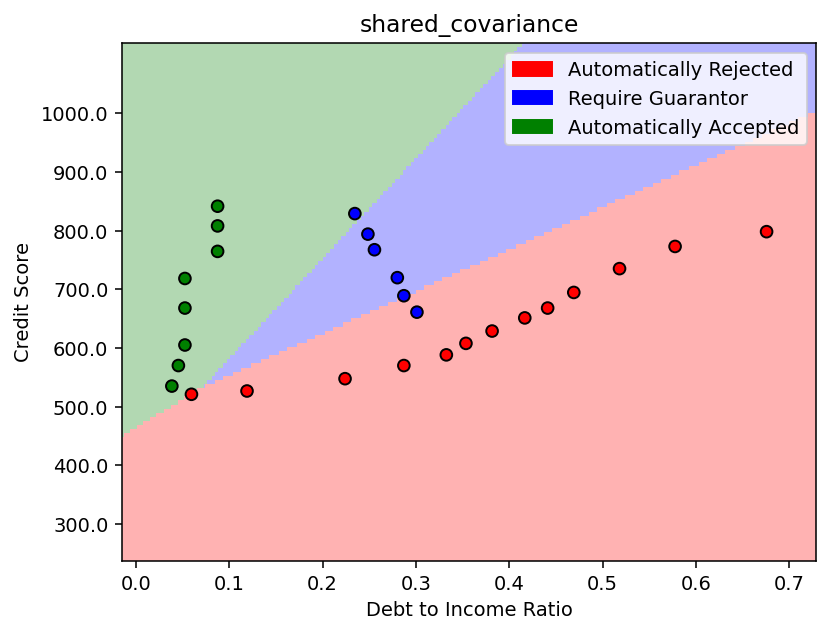
\includegraphics[width=\textwidth]{img_output/shared_covariance.png}\caption*{(a) Gaussian, shared covariance}\end{subfigure}
\begin{subfigure}{0.48\textwidth}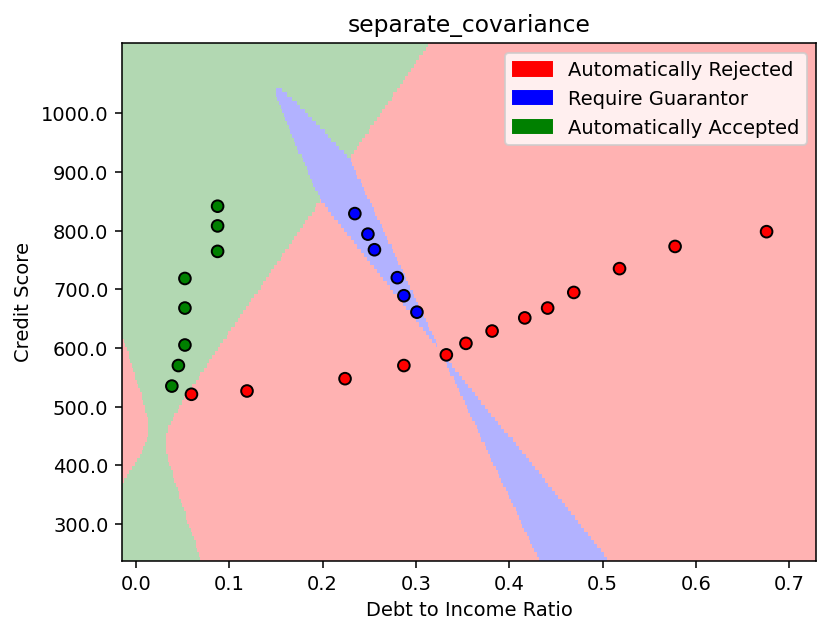
\includegraphics[width=\textwidth]{img_output/separate_covariance.png}\caption*{(b) Gaussian, separate covariances}\end{subfigure}
\\[2pt]
\begin{subfigure}{0.48\textwidth}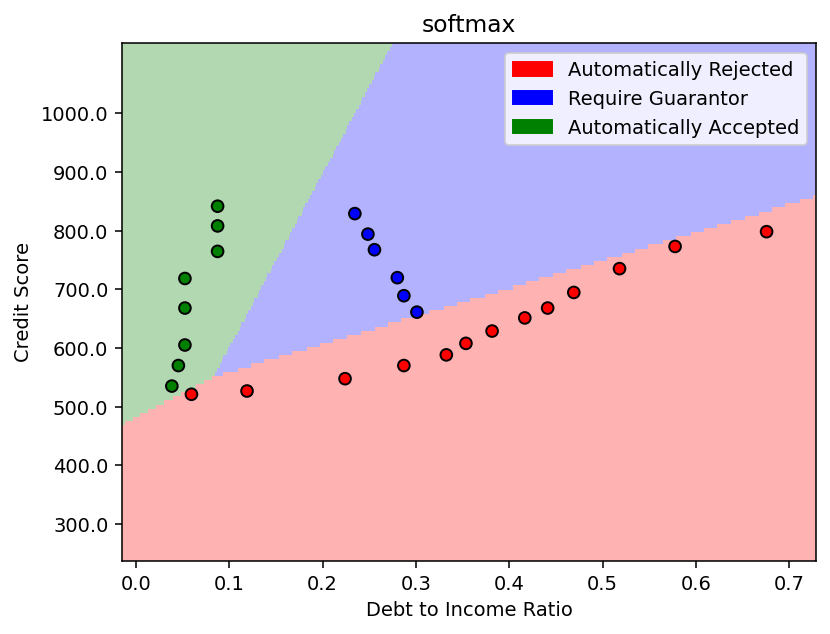
\includegraphics[width=\textwidth]{img_output/softmax.png}\caption*{(c) Softmax regression}\end{subfigure}
\begin{subfigure}{0.48\textwidth}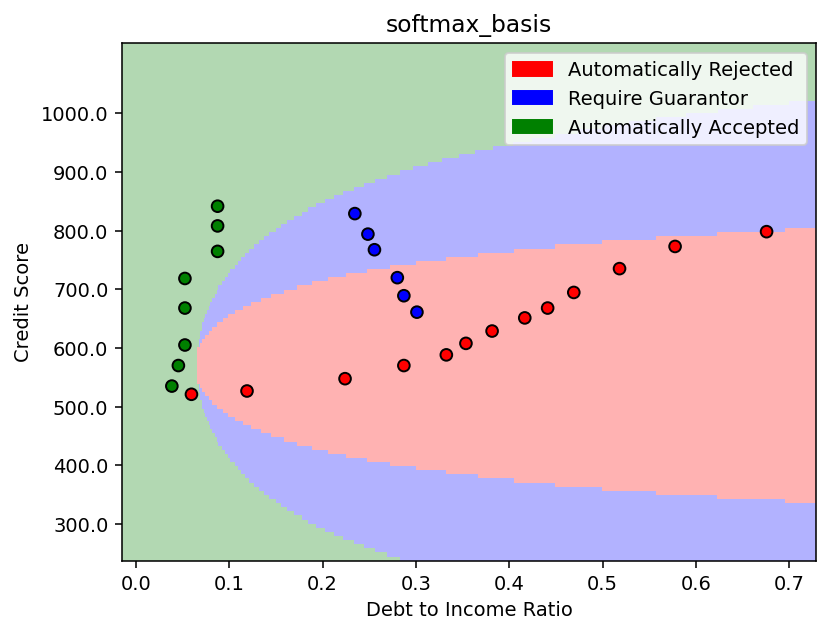
\includegraphics[width=\textwidth]{img_output/softmax_basis.png}\caption*{(d) Softmax with $\phi(\boldx)=[\ln(x_1{+}10),\,x_2^2]$}\end{subfigure}
\\[2pt]
\begin{subfigure}{0.48\textwidth}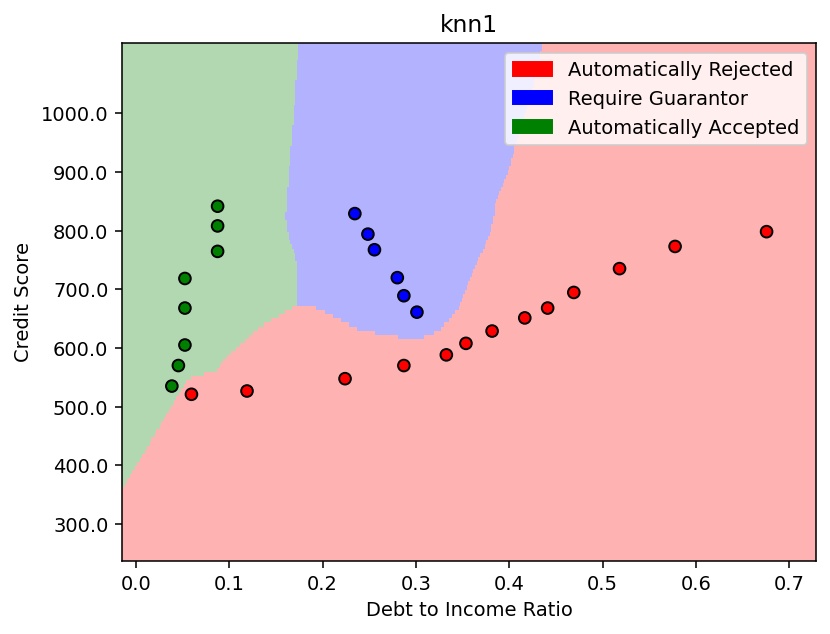
\includegraphics[width=\textwidth]{img_output/knn1.png}\caption*{(e) kNN, $k=1$}\end{subfigure}
\begin{subfigure}{0.48\textwidth}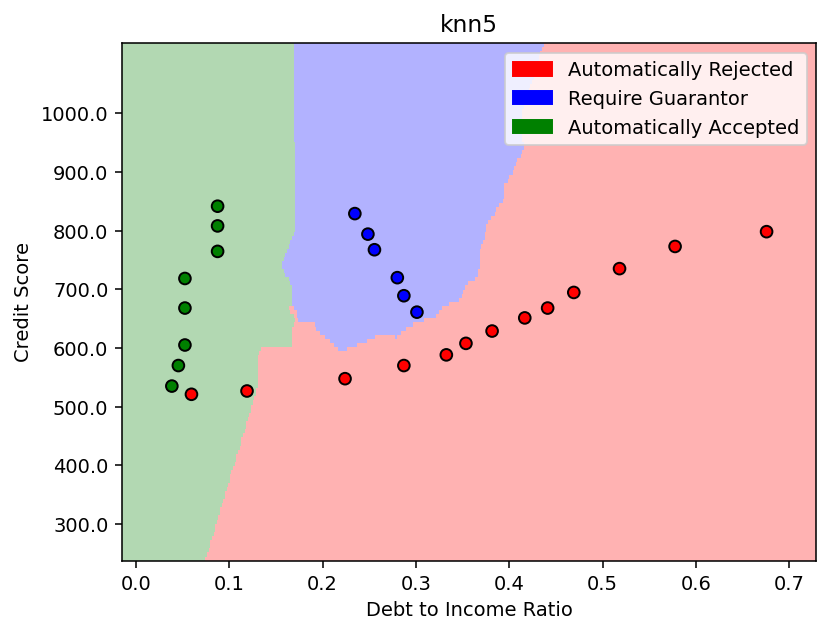
\includegraphics[width=\textwidth]{img_output/knn5.png}\caption*{(e) kNN, $k=5$}\end{subfigure}
\end{figure}

\noindent\textbf{Similarities.} All six recover the same coarse structure, which is
genuinely present in the data: low debt with high credit score is accepted (green,
upper left), high debt is rejected (red, right), and a thin band of intermediate
applicants requires a guarantor (blue). Every model separates the three training
clusters more or less correctly; they differ mainly in the \emph{shape} of the
boundaries and in what they do away from the data.

\noindent\textbf{Differences, and what causes them.} The decisive factor is the
functional form each model's decision rule is allowed to take.

\begin{itemize}
  \item \textbf{(a) Shared covariance $\Rightarrow$ exactly linear boundaries.} Taking the
    log-ratio of two class posteriors, the quadratic terms
    $-\tfrac12\boldx^\top\bSigma^{-1}\boldx$ are identical for both classes and cancel,
    leaving a function linear in $\boldx$. The result is a \emph{linear discriminant}:
    the plane is carved by straight lines meeting at a point. This is why (a) misses
    one training point --- straight lines simply cannot fence off the blue cluster here
    ($92.6\%$ training accuracy).

  \item \textbf{(b) Separate covariances $\Rightarrow$ quadratic (conic) boundaries.} With
    $\bSigma_k$ differing by class the quadratic terms no longer cancel, so the
    log-ratio is a quadratic form and the boundaries become conic sections --- visible
    as the curved wedge pinching the blue region into a narrow diagonal band. The extra
    flexibility costs parameters ($3$ covariance matrices instead of $1$), and with
    only $6$ points in the guarantor class the fitted $\bSigma_1$ is nearly singular,
    which is exactly why that band is so thin and elongated. It attains $100\%$
    training accuracy, but that band is a strong extrapolation from very little data.

  \item \textbf{(c) Softmax regression $\Rightarrow$ linear boundaries again, but fit
    discriminatively.} The decision rule compares $\boldw_k^\top\boldx$ across classes,
    so boundaries are again straight lines. Unlike (a), nothing is assumed about how
    the features are distributed --- the weights are chosen only to separate the
    classes, so the lines sit where they minimise classification loss rather than where
    two fitted Gaussians happen to cross. Here that is enough to reach $100\%$
    training accuracy where the generative linear model (a) could not.

  \item \textbf{(d) Softmax with the feature map $\Rightarrow$ curved boundaries.} The
    boundaries are still linear in $\phi(\boldx) = [\ln(x_1+10),\, x_2^2]$, but pulling
    that back to the original axes bends them. Because $x_2^2$ is symmetric about
    $x_2 = 0$, the model cannot distinguish a credit score above the centre from the
    mirrored one below, which destroys information the raw feature carried and drops
    training accuracy to $85.2\%$ --- a reminder that a basis expansion is not
    automatically an improvement.

  \item \textbf{(e) kNN $\Rightarrow$ piecewise-linear, non-parametric boundaries.} The
    boundary is a union of edges of the (distance-weighted) Voronoi diagram of the
    training points, so it is irregular and purely local. With $k=1$ it hugs the data
    exactly ($100\%$ training accuracy by construction) and is correspondingly jagged;
    with $k=5$ voting smooths it out, the green region shrinks, and training accuracy
    falls to $92.6\%$ --- the same bias--variance movement as Problem 1, with $k$ as
    the smoothing knob. The $1/9$ weight on the debt coordinate stretches distances
    along the credit-score axis, which is why the cells are elongated horizontally.
\end{itemize}

\noindent In short: \textbf{(a) and (c) are linear because their log-odds are linear in
$\boldx$; (b) and (d) curve because a quadratic enters (through unequal covariances and
through $x_2^2$ respectively); (e) is irregular because it fits no global function at
all.}

%%%%%%%%%%%%%%%%%%%%%%%%%%%%%%%%%%%%%%%%%%%%%%%%%%%%%%%%%%%%%%%%%%%%%% 3.2
\item
The applicant has debt-to-income ratio $0.32$ and credit score $350$, which the given
transformation maps to $\boldx^* = [1.6429,\, -1.5714]^\top$.

\begin{center}
\begin{tabular}{llc}
  \hline
  Model & Predicted class & Class probabilities $[\,\text{Rej},\ \text{Guar},\ \text{Acc}\,]$ \\
  \hline
  (a) shared covariance   & Automatically Rejected & $[1.000,\; 8.54\times10^{-7},\; 4.22\times10^{-10}]$ \\
  (b) separate covariance & Automatically Rejected & $[1.000,\; \approx 0,\; \approx 0]$ \\
  (c) softmax             & Automatically Rejected & $[1.000,\; 5.73\times10^{-23},\; 1.55\times10^{-33}]$ \\
  (d) softmax with $\phi$ & \textbf{Require Guarantor} & $[0.2197,\; \mathbf{0.7802},\; 7.21\times10^{-5}]$ \\
  (e) kNN, $k=1$          & Automatically Rejected & --- \\
  (e) kNN, $k=5$          & Automatically Rejected & --- \\
  \hline
\end{tabular}
\end{center}

\noindent Five of the six models say reject; only model (d) disagrees, and it does so
for a revealing reason --- its $x_2^2$ feature maps this very low credit score
($x_2 = -1.57$) to the same value as a high one ($x_2 = +1.57$), so the applicant is
confused with the well-qualified cluster. Each model reaches its decision differently:
the generative models (a) and (b) ask which class's fitted Gaussian makes
$\boldx^*$ most likely (weighted by the class prior); the discriminative models (c)
and (d) just evaluate which $\boldw_k^\top\boldx^*$ is largest; and kNN simply reads
off the labels of the nearest training applicants. The crucial thing to be aware of is
that this point lies \emph{far outside} the training data --- no training applicant has
a credit score near $350$ --- so every one of these numbers is an extrapolation. The
reported probabilities of $1.000$ and $10^{-33}$ are not evidence of certainty but an
artifact of the models' functional forms being extended into a region where no data
constrains them: softmax log-odds grow without bound as you move away from the
boundary, and Gaussian densities decay exponentially, so both produce arbitrarily
extreme confidence off the edge of the data. Exactly as in Problem 1.5, the honest
summary is high epistemic uncertainty masquerading as near-zero aleatoric uncertainty,
and the models' disagreement here (five to one) is a far better uncertainty signal than
any single model's probability.

%%%%%%%%%%%%%%%%%%%%%%%%%%%%%%%%%%%%%%%%%%%%%%%%%%%%%%%%%%%%%%%%%%%%%% 3.3
\item
There are several serious problems with deploying this classifier to make real lending
decisions.

\noindent\textbf{The training labels encode past human decisions, not ground truth.}
The target variable is the category a previous process assigned --- ``Automatically
Rejected'', ``Require Guarantor'', ``Automatically Accepted'' --- not whether the
applicant actually repaid. A model trained this way learns to \emph{reproduce the
lender's historical behaviour}, including any discrimination embedded in it. If past
officers systematically disfavoured applicants from particular neighbourhoods or
backgrounds, the classifier will reproduce that pattern while wrapping it in the
appearance of mathematical objectivity, and it will do so at scale and without the
possibility of a human exercising judgement. This also creates a feedback loop:
rejected applicants never generate repayment data, so the model's belief that they
were bad risks is never tested and the bias becomes self-confirming.

\noindent\textbf{Credit score and debt-to-income ratio are proxies, and imperfect
ones.} Both measure access to credit as much as creditworthiness. A graduate student
with high student debt and a thin credit file, a recent immigrant with no domestic
credit history, a person who has deliberately avoided debt, or someone whose score
collapsed after a one-off medical emergency or a period of unemployment would all score
badly here, yet many would repay reliably. Conversely, inherited wealth produces an
excellent score without indicating anything about the individual's discipline. Credit
scores also correlate with race, age, and geography in ways that are well documented,
so using them can produce disparate impact even though no protected attribute appears
in the feature vector --- omitting a variable does not make a model blind to it.

\noindent\textbf{The dataset is far too small, and the model is overconfident outside
it.} There are only $27$ training applicants, with just $6$ in the guarantor class.
As Problem 3.2 showed, the models then assign probabilities like $1.000$ and
$10^{-33}$ to a point no training data speaks to. Deploying a system that is this
confident this far from its evidence is indefensible when the consequence is denying
someone a loan.

\noindent\textbf{What would help.} Predict repayment rather than past approvals; audit
error rates separately across demographic groups rather than only overall accuracy;
include ability-to-pay variables such as income stability and employment history;
report calibrated uncertainty and abstain --- routing to human review --- when the
applicant falls outside the training distribution or the models disagree, as they did
in 3.2; and preserve a right to explanation and appeal. More broadly, a decision that
materially affects someone's life should keep a human accountable for it; the
classifier is at best a triage aid, and the ``Automatically'' in two of the three class
names is precisely the part that should be reconsidered.

\end{enumerate}
\end{solution}

\newpage

\begin{problem}[Gradient Descent and Regularization, 15pts]

\noindent In this problem, you will analyze gradient descent for linear regression and study how \emph{ridge regularization} modifies the optimization landscape. You will first derive gradient descent updates for ordinary least squares, then extend them to the ridge-regularized objective. Finally, you will implement these algorithms to empirically observe how regularization affects convergence and generalization.

\medskip

\noindent Consider a regression dataset $\mathcal D = \{(\mathbf x_i, y_i)\}_{i=1}^N$, where each input $\mathbf x_i \in \mathbb{R}^D$ and response $y_i \in \mathbb{R}$. Let $\mathbf X \in \mathbb{R}^{N \times D}$ denote the design matrix and let $\mathbf y \in \mathbb{R}^N$ denote the vector of responses.
\\\\
\textbf{Detail:} The predictors in this dataset are \emph{highly correlated}.
As a result, the ordinary least squares objective may be ill-conditioned,
which can lead to unstable gradient descent updates and high-variance
parameter estimates. In later parts of this problem, we will examine how
ridge regularization modifies the optimization landscape in this setting.
\\\\
\noindent Consider the ordinary least squares objective
\begin{equation*}
    \mathcal L(\mathbf w) = \frac{1}{2} \|\mathbf X\mathbf w - \mathbf y\|_2^2.
\end{equation*}

\begin{enumerate}

\item Derive the gradient $\nabla_{\mathbf w} \mathcal L(\mathbf w)$ with respect to the parameter vector $\mathbf w$. Your final expression should be written in matrix/vector form and simplified as much as possible.

\item Using your result, write the full-batch gradient descent update rule for
$\mathbf w$ with step size $\eta > 0$.
\\\\
\noindent Now consider the ridge-regularized objective
\begin{equation*}
    \mathcal L_\text{ridge}(\mathbf w) = \frac{1}{2} \|\mathbf X\mathbf w - \mathbf y\|_2^2 + \frac{\lambda}{2} \|\mathbf w\|_2^2,
\end{equation*}
where $\lambda \ge 0$ is a regularization parameter. Important note: typically, we do not regularize the bias term, $w_0$, thus $\|\mathbf w\|_2^2$ should be replace with $\mathbf w'$ where $w'_0 = 0$. However, for the sake of simplicity, we will omit that detail for the rest of the problem.

\item Derive the gradient $\nabla_{\mathbf w}\mathcal L_\text{ridge}(\mathbf w)$. Clearly indicate how the regularization term modifies the gradient compared to the unregularized case.


\item Rewrite the update in a form that makes the effect of ridge regularization
explicit. Briefly explain how this form illustrates the shrinkage effect of the
regularization term on the parameters.

\item You will implement gradient descent for both the ordinary least squares and
ridge-regularized objectives derived above and empirically study the effect of
regularization. Specifically, you will

\begin{itemize}
    \item Implement gradient and loss functions for both regular and ridge regression
    \item Write update step functions for stochastic gradient descent, stochastic gradient descent + momentum, and Adam optimizer.
\end{itemize}

Try not to touch anything that is not in between ``\textit{sol}" and ``\textit{los}"!


\item Generate the contour plots for the trajectories of the three algorithms across both the regularized and non-regularized case. What do you notice about the speed of convergence as well as where the algorithms converge to? What do you notice about the geometry of the loss function?\\
\textit{Note: the graphing code will pause when the first descent converges, so we see that some will not converge. Also, you'll see a subspace for the optimum in the unregularized case since we have a non-full rank data matrix $\mathbf X$!}

\end{enumerate}
\end{problem}

\pagebreak

\begin{solution}
\begin{enumerate}

%%%%%%%%%%%%%%%%%%%%%%%%%%%%%%%%%%%%%%%%%%%%%%%%%%%%%%%%%%%%%%%%%%%%%% 4.1
\item
Expand the objective as an inner product:
\[
  \mathcal L(\boldw) = \tfrac12\|\boldX\boldw - \boldy\|_2^2
  = \tfrac12(\boldX\boldw-\boldy)^\top(\boldX\boldw-\boldy)
  = \tfrac12\Big(\boldw^\top\boldX^\top\boldX\boldw - 2\boldy^\top\boldX\boldw + \boldy^\top\boldy\Big).
\]
Using $\nabla_{\boldw}(\boldw^\top \mathbf A\boldw) = 2\mathbf A\boldw$ for symmetric
$\mathbf A = \boldX^\top\boldX$, and $\nabla_{\boldw}(\boldb^\top\boldw) = \boldb$,
\[
  \boxed{\;\nabla_{\boldw}\mathcal L(\boldw) = \boldX^\top\boldX\boldw - \boldX^\top\boldy
   = \boldX^\top(\boldX\boldw - \boldy)\;}
\]

%%%%%%%%%%%%%%%%%%%%%%%%%%%%%%%%%%%%%%%%%%%%%%%%%%%%%%%%%%%%%%%%%%%%%% 4.2
\item
Full-batch gradient descent steps against the gradient with step size $\eta > 0$:
\[
  \boxed{\;\boldw^{(t+1)} = \boldw^{(t)} - \eta\,\boldX^\top\big(\boldX\boldw^{(t)} - \boldy\big)\;}
\]
Equivalently $\boldw^{(t+1)} = (\boldI - \eta\boldX^\top\boldX)\boldw^{(t)} + \eta\boldX^\top\boldy$,
which converges iff $0 < \eta < 2/\lambda_{\max}(\boldX^\top\boldX)$.

%%%%%%%%%%%%%%%%%%%%%%%%%%%%%%%%%%%%%%%%%%%%%%%%%%%%%%%%%%%%%%%%%%%%%% 4.3
\item
The penalty is separable from the data term, so the gradients simply add. With
$\nabla_{\boldw}\big(\tfrac{\lambda}{2}\|\boldw\|_2^2\big) = \lambda\boldw$,
\[
  \boxed{\;\nabla_{\boldw}\mathcal L_{\text{ridge}}(\boldw)
   = \underbrace{\boldX^\top(\boldX\boldw-\boldy)}_{\text{unregularized gradient}} + \underbrace{\lambda\boldw}_{\text{new term}}\;}
\]
The regularizer contributes a term pointing from $\boldw$ straight back toward the
origin, with magnitude proportional to $\|\boldw\|$. Geometrically it adds
$\lambda\boldI$ to the Hessian, turning $\boldX^\top\boldX$ into
$\boldX^\top\boldX + \lambda\boldI$: every eigenvalue is lifted by $\lambda$, so even
the flat directions of the OLS objective acquire positive curvature.

%%%%%%%%%%%%%%%%%%%%%%%%%%%%%%%%%%%%%%%%%%%%%%%%%%%%%%%%%%%%%%%%%%%%%% 4.4
\item
Substituting the ridge gradient into the update and collecting the $\boldw^{(t)}$ terms:
\[
  \boldw^{(t+1)}
  = \boldw^{(t)} - \eta\Big[\boldX^\top(\boldX\boldw^{(t)}-\boldy) + \lambda\boldw^{(t)}\Big]
  \;=\;
  \boxed{\;(1-\eta\lambda)\,\boldw^{(t)} \;-\; \eta\,\boldX^\top\big(\boldX\boldw^{(t)}-\boldy\big)\;}
\]
Written this way the effect is explicit: \textbf{each iteration first multiplies the
entire weight vector by the constant $(1-\eta\lambda) < 1$ --- shrinking it uniformly
toward the origin --- and then applies the ordinary least-squares step.} This is why
ridge regularization is also called \emph{weight decay}: absent any data signal, the
weights decay geometrically as $(1-\eta\lambda)^t \to 0$. The fixed point is reached
where the shrinkage pull exactly balances the data's pull, which happens strictly
closer to the origin than the OLS solution. Note also that the shrinkage is largest in
directions where the data provides least evidence: along an eigenvector of
$\boldX^\top\boldX$ with eigenvalue $s$, the solution is scaled by $s/(s+\lambda)$, so
well-determined directions ($s \gg \lambda$) are barely touched while poorly
determined ones ($s \ll \lambda$) are suppressed almost entirely.

%%%%%%%%%%%%%%%%%%%%%%%%%%%%%%%%%%%%%%%%%%%%%%%%%%%%%%%%%%%%%%%%%%%%%% 4.5
\item
Implemented in the notebook. The loss and gradient functions follow the docstrings'
$1/n$ normalisation,
\[
  \mathcal L(\boldw) = \frac{1}{2n}\|\boldX\boldw-\boldy\|_2^2, \quad
  \nabla \mathcal L = \frac1n \boldX^\top(\boldX\boldw-\boldy), \quad
  \nabla\mathcal L_{\text{ridge}} = \nabla\mathcal L + \lambda\boldw,
\]
and the three optimizers implement
\begin{align*}
  \text{SGD:}      &\quad \boldw_{t+1} = \boldw_t - \eta\,\boldg_t \\
  \text{Momentum:} &\quad \boldv_{t+1} = \beta\boldv_t + \boldg_t, \qquad \boldw_{t+1} = \boldw_t - \eta\,\boldv_{t+1} \\
  \text{Adam:}     &\quad \boldm_t = \beta_1\boldm_{t-1} + (1-\beta_1)\boldg_t, \quad
                          \boldv_t = \beta_2\boldv_{t-1} + (1-\beta_2)\boldg_t^2, \\
                   &\quad \hat\boldm_t = \tfrac{\boldm_t}{1-\beta_1^t}, \quad
                          \hat\boldv_t = \tfrac{\boldv_t}{1-\beta_2^t}, \qquad
                          \boldw_{t+1} = \boldw_t - \eta\,\tfrac{\hat\boldm_t}{\sqrt{\hat\boldv_t}+\epsilon}.
\end{align*}

%%%%%%%%%%%%%%%%%%%%%%%%%%%%%%%%%%%%%%%%%%%%%%%%%%%%%%%%%%%%%%%%%%%%%% 4.6
\item
\begin{center}
  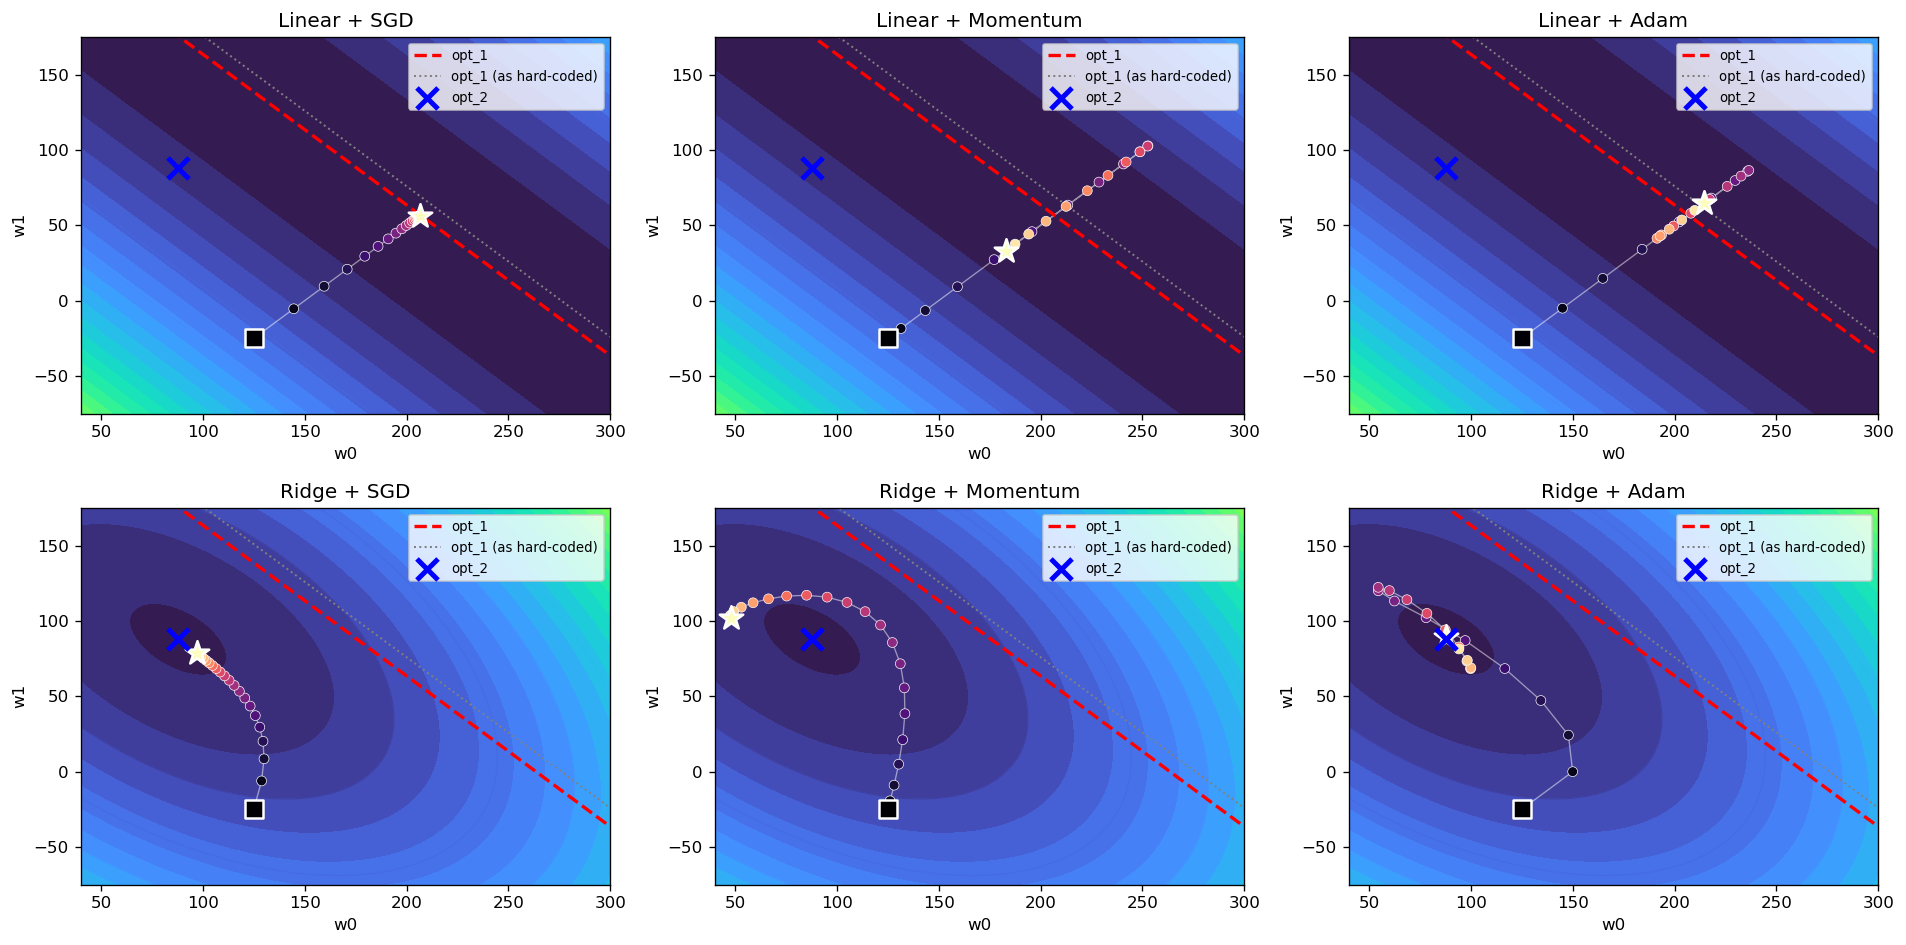
\includegraphics[width=\textwidth]{img_output/p4.6_contours.png}
\end{center}

\noindent\textbf{The geometry of the loss.} The generating code sets
$x_1 = 0.12\,x_0$ exactly, so after standardisation the two columns of $\boldX$ become
\emph{identical}. The design matrix has rank $1$ (singular values $15.49$ and $0$), and
$\boldX^\top\boldX/n$ has eigenvalues $\{0, 2\}$ --- infinite condition number. Since
the prediction depends on $\boldw$ only through the sum $w_0 + w_1$, the unregularized
loss is completely flat along the direction $(1,-1)$ and curved only along $(1,1)$.
The top row therefore shows a \emph{trough}, not a bowl: the minimum is an entire line
rather than a point, which is the ``subspace of optima'' the problem note refers to.
The level sets are parallel straight bands, and gradients are everywhere perpendicular
to them, so no optimizer can move along the valley floor --- where along the line it
stops depends entirely on where it started. Adding $\lambda = 1$ lifts both eigenvalues
to $\{1, 3\}$, collapsing the condition number from $\infty$ to $3$. The bottom row is
accordingly a proper elliptical bowl with a single well-defined minimum.

\noindent\textbf{Where they converge.} The OLS optima form the line
$w_0 + w_1 = 263.55$, while ridge has the unique optimum
$\boldw^* = [87.85,\, 87.85]^\top$, i.e.\ $w_0 + w_1 = 175.70$ --- shrunk by
$33.3\%$ toward the origin, exactly the effect derived in part 4. Ridge also resolves
the degeneracy by picking the minimum-norm point on (near) the valley, splitting the
total weight evenly between the two identical features rather than leaving the split
arbitrary. So regularization buys two things here at once: a well-conditioned,
fast-converging problem, and a unique, stable answer in a setting where the
unregularized problem has no unique answer at all.

\noindent\textbf{Speed of convergence.} After the $20$ allotted steps:
\begin{center}
\begin{tabular}{lccc}
  \hline
  Run & Final $\boldw$ & Distance to optimum & Final loss \\
  \hline
  Linear $+$ SGD      & $[206.44,\ 56.44]$ & $0.478$  & $0.236$ \\
  Linear $+$ Momentum & $[183.06,\ 33.06]$ & $33.543$ & $1125.142$ \\
  Linear $+$ Adam     & $[214.62,\ 64.62]$ & $11.099$ & $123.196$ \\
  \hline
  Ridge $+$ SGD       & $[96.94,\ 78.70]$  & $12.895$ & $11659.695$ \\
  Ridge $+$ Momentum  & $[48.20,\ 101.67]$ & $41.994$ & $12791.919$ \\
  Ridge $+$ Adam      & $[88.06,\ 89.46]$  & $\mathbf{1.618}$ & $\mathbf{11579.496}$ \\
  \hline
\end{tabular}
\end{center}
\noindent (For the linear runs ``distance'' is the perpendicular distance to the line
of optima, since every point on it is equally optimal; the optimal ridge loss is
$11576.550$.) Plain SGD descends monotonically and lands essentially on the valley
floor in the unregularized case. Momentum is the \emph{worst} performer in both rows:
its velocity term keeps accumulating along the single curved direction and it
overshoots badly, oscillating back and forth --- the distance to the optimum goes
$115.6 \to 41.8 \to 48.0 \to 59.4 \to 8.2 \to 33.5$ rather than decreasing steadily.
Adam makes the fastest early progress (down to $6.4$ after only $4$ steps in the linear
case) because its per-coordinate rescaling by $\sqrt{\hat v}$ makes it nearly invariant
to the terrible conditioning, and it finishes closest of the three on the ridge
objective. Its path is visibly jittery because $\beta_2 = 0.8$ gives a very short
second-moment memory. The overall lesson matches the problem's framing: on an
ill-conditioned, ravine-shaped objective the choice of optimizer matters a great deal,
and conditioning the problem itself through regularization is at least as effective as
switching optimizer.

\noindent\emph{One note on the provided plotting code:} the red dashed reference line
is drawn at $w_0 + w_1 = 276$, whereas the true line of OLS optima for this data is
$w_0 + w_1 = 263.55$. The dashed line in the figures therefore sits slightly above the
actual optimum; the fitted values reported in the table use the true optimum.

\end{enumerate}
\end{solution}


%%%%%%%%%%%%%%%%%%%%%%%%%%%%%%%%%%%%%%%%%%%%%
% Name and Calibration
%%%%%%%%%%%%%%%%%%%%%%%%%%%%%%%%%%%%%%%%%%%%%

\pagebreak
\textbf{Name}:

\textbf{Collaborators and Resources}:

\end{document}
